\documentclass[./\jobname.tex]{subfiles}
\begin{document}

\chapter{Problem Definition}
This chapter describes the broader idea of the \gls{wrm}, which is used to reformulate any differential equation into an optimisation problem, and its application in the field of spectral methods (\cite{shen_spectral_2011}). The fitness function originates from these approaches. Further, the different approximation schemes and numerical solution representation are depicted. The following paragraphs also introduce the mathematical notation used for this work. 

\section{Theoretical Foundation}
\label{chap:opt_problem}

The most general description of a \gls{pde} is displayed in equation \ref{eq:general_pde}.
\begin{equation}
\label{eq:general_pde}
\begin{split}
\mathbf{L}u(\mathbf{x}) & = f(\mathbf{x}) \\
\text{subjected to: }\mathbf{B}u(\mathbf{x}) & = g(\mathbf{x}) \\
\end{split}
\end{equation}
This is similar to the formulation of the strong form in equantion \ref{eq: strong form}, but not limited to a Dirichlet boundary problem. The matrix $\mathbf{B}$ can include differentiation, effectively allowing i.e. Neumann boundary condition. 

An approximate solution to this problem is expressed as a finite sum of basis functions $\phi_k(\mathbf{x})$, as denoted in equation \ref{eq:u_apx}. The coefficients $a_k$ are to be determined. In classical approximation schemes, the basis functions are orthogonal, such as trigonometric functions or Lagrange basis polynomials. 

\begin{equation}
\label{eq:u_apx}
u(\mathbf{x}) \approx u_{apx}(\mathbf{x}) = \sum_{k=0}^{N} a_k \phi_k (\mathbf{x})
\end{equation}

The residual of a \gls{pde}, as shown in equation \ref{eq:residual}, is formulated as the difference between the left and the right side of the equation. The residual of a solved \gls{pde} is zero. This is only possible for the $u_{ext}(x,y)$ analytical solution. For a numerical approximation $u_{apx}(x,y)$, the residual should be ''small enough``. 

\begin{equation}
\label{eq:residual}
\mathbf{R}(\mathbf{x}) = \mathbf{L}u_{apx}(\mathbf{x}) - f(\mathbf{x})
\end{equation}

The \gls{wrm} (\cite{shen_spectral_2011}) tries to minimise this resiual of a numerical candidate solution over the whole domain $\Omega$. Therefore, $R$ at every $\mathbf{x}_i \in \Omega$ is evaluated and added up, resulting in the following integral of equation \ref{eq:wrm}. The residual at every $\mathbf{x}$ can be scaled by a weighting function over the domain as denoted with $W(\mathbf{x})$. The choice of the test function $\psi(\mathbf{x})$ is distinct for different methods. The actual optimum does not change, since the zero-product property holds. The \gls{wrm} builds the basis for many solving strategies, including \gls{fem}. 

\begin{equation}
\label{eq:wrm}
WRF = \int_{\Omega} \mathbf{R}(\mathbf{x}) \psi(\mathbf{x}) W(\mathbf{x}) dx
\end{equation}

This integral must be evaluated numerically. There are many different integration schemes available, but they are typically computational expensive. A less extensive approach is to evaluate the integral argument at different ``collocation points'' and add up the results. This can be seen in equation \ref{eq:wrm_colloc}. Although it is not an integral per se, it does assign a numerical ``score'' to the residual. 

\begin{equation}
\label{eq:wrm_colloc}
\sum_{k=0}^{N} \mathbf{R}(\mathbf{x}_k) \psi(\mathbf{x}_k) W(\mathbf{x}_k)
\end{equation}

To ensure, that negative and positive residuals do not get canceled out, a common choice in heuristic methods from table \ref{tab:results_literature_comparison}, is to choose $\psi(\mathbf{x}_k)$ as the residual itself, effectively squaring it. The resulting ``sum of squared residuals'' forms the basis for nearly all fitness function in the current literature, as represented in equation \ref{eq:sum_squared_residual}.

\begin{equation}
\label{eq:sum_squared_residual}
\sum_{k=0}^{N} \mathbf{R}(\mathbf{x}_k)^2 W(\mathbf{x}_k)
\end{equation}

These methods are often called ``spectral methods'' (\cite{shen_spectral_2011}). Their main advantage over finite difference methods is, that they take the whole domain into account. The derivative of the function at one point is influenced by the function at every other point in the domain. This global approch can lead to a better accuracy. 

\section{Fitness Function}
\label{chap:fit_func}

As mentioned above, the basis of the fintess function used in \cite{chaquet_using_2019} is the squared weighted residual in equation \ref{eq:sum_squared_residual}. They split the summation over the collocation points into two parts: the points on the boundary ($nb$) and the points on the inner domain ($nc$). Further, they devide the fitness value by the number of points used. This fitness function, as seen in equation \ref{eq:fit_func}, is adopted in this work. 

\begin{equation}
\label{eq:fit_func}
F(u_{apx}) = \frac{\sum_{i=1}^{n_C} \xi (\mathbf{x}_i) || \mathbf{L}u(\mathbf{x}_i) - f(\mathbf{x}_i)||^2 + \phi \sum_{j=1}^{n_B} || \mathbf{B}u(\mathbf{x}_j) - g(\mathbf{x}_j)||^2}{(n_C + n_B)}  
\end{equation}

The fitness function has two important properties: 
\begin{itemize}
	\item The fitness value of the exact solution must be 0:\\
	$F(u_{ext}(\mathbf{x})) \equiv 0$ 
	\item The fitness value of an approximate solution is greater or equal to 0: \\
	$F(u_{apx}(\mathbf{x})) \geq 0$
\end{itemize}
 

The weighting function is also split into two parts: $\xi$ for the inner collocation points and $\phi$ as penalty factor for the boundary points. The weighting function $\xi$ can be adapted by a parameter $\kappa$. For a $\kappa > 1$, $\xi$ assigns larger values for collocation points closer to the boundary, effectively shifting the relative importance towards the boundary. These weights can be calculated apriori, so no computational effort is added to the fitness function. Again, the weights are directly extracted from \cite{chaquet_using_2019}. 

\begin{equation}
\label{eq:nc_weight}
\xi(\mathbf{x}_i) = \frac{1 + \kappa \left(1 - \frac{min_{\forall \mathbf{x}_j\in n_B}|| \mathbf{x}_i - \mathbf{x}_j ||}{max_{\forall\mathbf{x}_k \in n_C}(min_{\forall \mathbf{x}_j \in n_B} || \mathbf{x}_k - \mathbf{x}_j ||)}\right)}{1 + \kappa}
\end{equation}


\section{Candidate Representation}
\label{chap:candidate_rep}

As \cite{chaquet_using_2019} suggest, an approximate solution should be represented as a summation of $N$ scaled and shifted radial basis functions $\phi$, as denoted in equation \ref{eq:u_apx} \todo{cite approximation theorem} \gls{rbf} are functions that only are point symmetric to a centre $c$ and their function value only depend on the radius $r$. 

\begin{equation}
\label{eq: radius}
\mathbf{r} = \left|\left|\mathbf{x} - \mathbf{c} \right|\right|
\end{equation}

This thesis mainly works with two different types of \gls{rbf}. The first one is the classical Gauss \gls{rbf} ($gak$). The second one, further called GSin \gls{rbf} ($gsk$), is more complex. A candidate solution is represended as the parameters that shift and deform these \gls{rbf}. 

\subsection{Gauss Kernel}
\label{chap:gauss_kernel}

The general Gauss kernel is the classical choice to approximate functions. It was first introduced in \cite{broomhead_multivariable_1988}. These kernels have been used in many different works, including \cite{chaquet_using_2019}. \todo{cite approximation proof} Equation \ref{eq:gauss_kernel} shows the formulation of such a kernel. One kernel has 4 parameters, that change its shape and location. $\omega$ is a scaling factor for each and $\gamma$ describes how sharp the e-function is. Depending on the space the solution is defined in, the number of $\mathbf{c}$ could change - one for each dimension. However, in this work only $\mathbf{R}^2$ is of interest. In figure \ref{fig:gauss_kernel_3d_plot} a single standard Gauss kernel is plotted. 

\begin{equation}
\label{eq:gauss_kernel}
gak(\mathbf{x}) = \omega e^{-\gamma \mathbf{r}^2}
\end{equation}

\begin{figure}[H]
	\centering
	\noindent\adjustbox{max width=\linewidth}{
		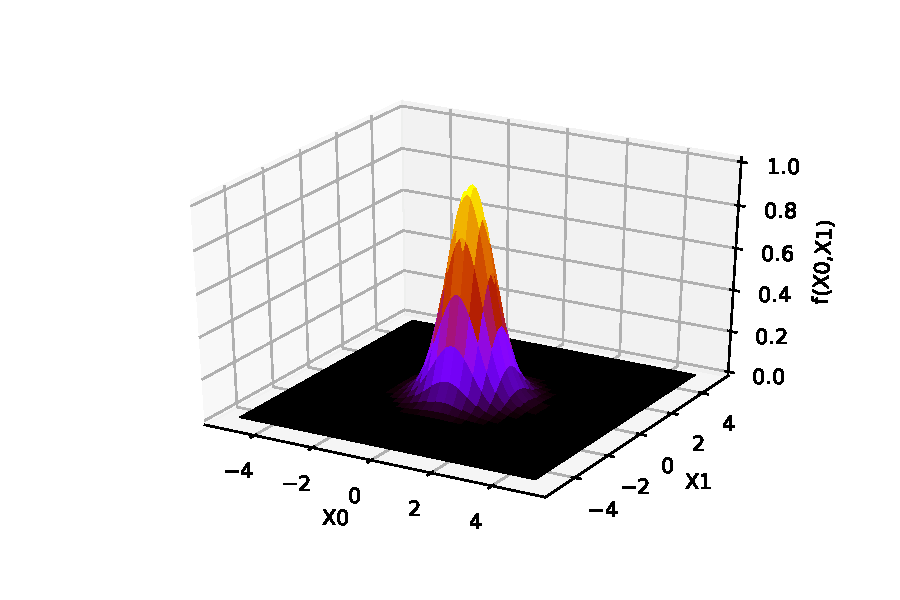
\includegraphics[width=\textwidth]{../../code/kernels/gak.pdf}
	}
	\unterschrift{3D plot of a single Gauss kernel with the parametes $\omega = 1$, $\gamma = 1$, $c_0 = 0$ and $c_1 = 0$}{}{}
	\label{fig:gauss_kernel_3d_plot}
\end{figure}

An approximate solution to the \gls{pde} in question is be described as the superposition of $N$ kernels as shown in equation \ref{eq:uapx_gauss_kernel}. 

\begin{equation}
\label{eq:uapx_gauss_kernel}
u_{apx}(\mathbf{x}) = \sum_{i=0}^{N} \omega_i e^{-\gamma_i \mathbf{r}_i^2}
\end{equation}

A solution is encoded as a vector of these $4\cdot N$ parameters stacked together. This is shown in eqution \ref{eq:gauss_parameter_vector}. 

\begin{equation}
\label{eq:gauss_parameter_vector}
\vec{u_{apx}} = \left[\underbrace{\omega_0, \gamma_0, c_{00}, c_{01}}_{\text{kernel 0}}, \cdots \underbrace{\omega_i, \gamma_i, c_{i0}, c_{i1}}_{\text{kernel i}}, \cdots \underbrace{\omega_N, \gamma_N, c_{N0}, c_{N1}}_{\text{kernel N}} \right]^T
\end{equation}

To evaluate the residual of a \gls{pde}, the derivatives must be known. To that extend, the derivative of $u_{apx}$ from equation \ref{eq:u_apx} is calculated. The first order derivative with respect to $x_0$ is seen in equation \ref{eq:uapx_gauss_kernel_x0}. To solve the proposed testbed, also the second order derivatives are needed, as described in equation \ref{eq:uapx_gauss_kernel_x0x0}. Although the mixed term derivative is not used in this work, for the sake of completeness it is displayed in equation \ref{eq:uapx_gauss_kernel_x0x1}.  


\begin{equation}
\label{eq:uapx_gauss_kernel_x0}
\frac{\partial u_{apx}(\mathbf{x})}{\partial x_0} = -2 \sum_{i=0}^{N} \omega_i \gamma_i (x_0 - c_{i0}) e^{-\gamma_i \mathbf{r}_i^2}
\end{equation}

\begin{equation}
\label{eq:uapx_gauss_kernel_x0x0}
\frac{\partial^2 u_{apx}(\mathbf{x})}{\partial x_0^2} = \sum_{i=0}^{N} \omega_i \gamma_i \left[ 4 \gamma_i (x_0 - c_{i0})^2 - 2 \right] e^{-\gamma_i \mathbf{r}_i^2}
\end{equation}

\begin{equation}
\label{eq:uapx_gauss_kernel_x0x1}
\frac{\partial^2 u_{apx}(\mathbf{x})}{\partial x_0 x_1} = 4 \sum_{i=0}^{N} \omega_i \gamma_i^2 (x_0 - c_{i0}) (x_1 - c_{i1}) e^{-\gamma_i \mathbf{r}_i^2} 
\end{equation}

\subsection{GSin Kernel}
\label{chap:gsin_kernel}
Additional to the Gauss kernel, a ``GSin'' kernel is proposed. \todo{approximation proof possible?}In essence, this is a multiplication of a Gauss kernel with a sine function, as seen in equation \ref{eq:gsin_kernel}. It can be thought of a sine function, where its influence declines with the radius $r$. Both ``sub-functions'' are centered at the same $\mathbf{c}$. 
The plot in figure \ref{fig:gsin_kernel_3d_plot} shows how the first half period is much larger than the second half. With the sine, two new parameters are introduced: $f$ for the frequency of the sine wave and $\varphi$ represents the phase shift. 
\begin{equation}
\label{eq:gsin_kernel}
gsk(\mathbf{x}) = \omega e^{-\gamma \mathbf{r}^2} sin(f \mathbf{r}^2 - \varphi)
\end{equation}

It is important to notice that, with the correct parameter choice, both traits - the sine and the e-function - can be retrieved. When $\gamma=0$ the e-function evaluates to 1 and leaves the sine on its own. By setting $f=0$ and $\varphi=\frac{\pi}{2}$, the sine vanishes and the e-function part is obtained. Thus, with this kernel, it should be possible to approximate the \gls{pde}s 0A and 0B from the testbed arbitrarily close. 

\begin{figure}[H]
	\centering
	\noindent\adjustbox{max width=\linewidth}{
		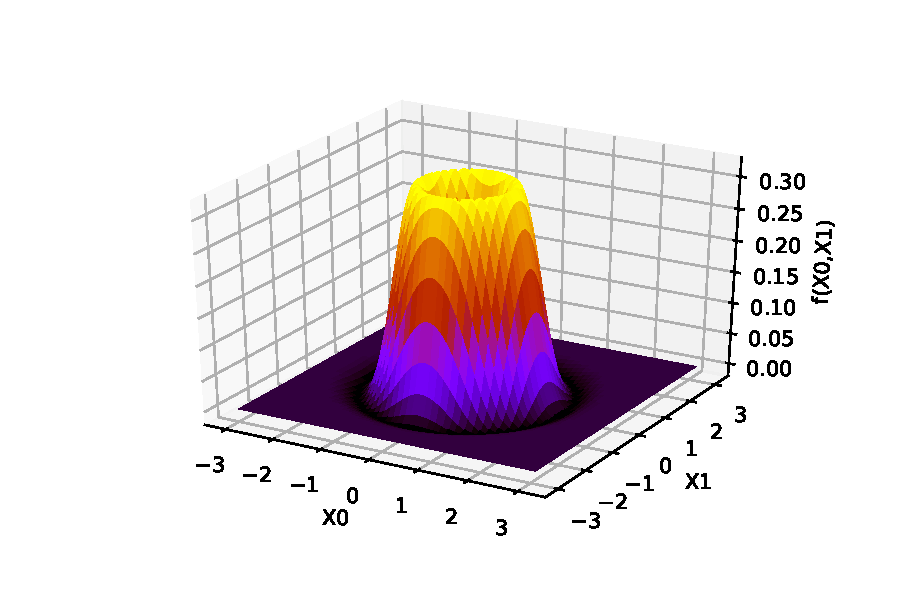
\includegraphics[width=\textwidth]{../../code/kernels/gsk.pdf}
	}
	\unterschrift{3D plot of a single GSin kernel with the parametes $\omega = 1$, $\gamma = 1$, $c_0 = 0$, $c_1 = 0$, $f = 1$, $\varphi = 0$}{}{}
	\label{fig:gsin_kernel_3d_plot}
\end{figure}

Similar to the Gauss kernel, the approximate solution is described as the superposition of $N$ GSin kernels, as seen in equation \ref{eq:uapx_gsin_kernel}. 

\begin{equation}
\label{eq:uapx_gsin_kernel}
u_{apx}(\mathbf{x}) = \sum_{i=0}^{N} \omega_i e^{\gamma_i \mathbf{r}_i^2} sin(f_i \mathbf{r}_i^2 - \varphi_i)
\end{equation}

Equation \ref{eq:gsin_parameter_vector} shows the solution representation in stacked vector notation, including the two new parameters $f$ and $\varphi$. 

\begin{equation}
\label{eq:gsin_parameter_vector}
\vec{u_{apx}} = \left[\underbrace{\omega_0, \gamma_0, c_{00}, c_{01}, f_0, \varphi_0}_{\text{kernel 0}}, \cdots \underbrace{\omega_i, \gamma_i, c_{i0}, c_{i1}, f_i, \varphi_i}_{\text{kernel i}}, \cdots \underbrace{\omega_N, \gamma_N, c_{N0}, c_{N1}, f_N, \varphi_N}_{\text{kernel N}} \right]^T
\end{equation}

Again, the derivatieves of the solution are needed, which are shown in the equations \ref{eq:uapx_gsin_kernel_x0} through \ref{eq:uapx_gsin_kernel_x0_x1}. 

\begin{equation}
\label{eq:uapx_gsin_kernel_x0}
\frac{\partial u_{apx}(\mathbf{x})}{\partial x_0} = \sum_{i=0}^{N} 2 \omega_i (x_0 - c_{i0}) e^{-\gamma_i \mathbf{r}_i^2} (\gamma_i sin(\varphi_i - f_i \mathbf{r}_i^2) + f_i cos(\varphi_i - f_i \mathbf{r}_i^2))
\end{equation}

\begin{equation}
\label{eq:uapx_gsin_kernel_x0_x0}
\begin{split}
& \frac{\partial^2 u_{apx}(\mathbf{x})}{\partial x_0^2} = \sum_{i=0}^{N} 2 \omega_i e^{-\gamma_i \mathbf{r}_i^2} \\ & [ (2 c_{i0}^2 (f_i^2 - \gamma_i^2) + 4 c_{i0} x (\gamma_i^2 - f_i^2) + 2 f_i^2 x^2 - 2 \gamma_i^2 x^2 + \gamma_i) sin(\varphi_i - f_i \mathbf{r}_i^2) + \\ & f_i (-4 c_{i0}^2 \gamma_i + 8 c_{i0} \gamma_i x - 4 \gamma_i x^2 + 1) cos(\varphi_i - f_i \mathbf{r}_i^2) ]
\end{split}
\end{equation}

\begin{equation}
\label{eq:uapx_gsin_kernel_x0_x1}
\begin{split}
& \frac{\partial^2 u_{apx}(\mathbf{x})}{\partial x_0 x_1} = \sum_{i=0}^{N}  4 \omega_i (c_{i0} - x) (c_{i1} - y) e^{-\gamma_i \mathbf{r}_i^2} \\ & \left[(f_i^2 - \gamma_i^2) sin(\varphi_i - f_i \mathbf{r}_i^2) - 2 f_i \gamma_i cos(\varphi_i - f_i \mathbf{r}_i^2)\right]
\end{split}
\end{equation}

\end{document}